\newpage
\section{細径MPAを用いた歩脚ロボットの開発}
本章では本研究で用いた改良した細径MPAの作製方法,それを用いた羽状筋の再現方法について述べる.
%%%%%%%%%%%%%%%%%%%%%%%%%%%%%%%%%%%%%%%%%%%%%%%%%%%%%%%%%
\subsection{羽状筋再現方法}
\subsubsection{細径MPA作製方法}
本研究で用いる3 mmの細径MPAの作製方法について説明する.
構造は2.1節で述べた従来のMPAと同様,シリコンゴムチューブをナイロン繊維メッシュで覆ったシンプルなもので,0.4~0.6 MPaで駆動し収縮率は約20 %である.
おおまかな作製手順を図\ref{fig:shingata_sakuseihouhou}に示す.
端部の締結方法はOリングを用いる方法を採用した.
図中\textcircled{\scriptsize 1}に示した物品が作製に必要なもので左から以下の通りである.
%
\begin{itemize}
  \item PPX(瞬間接着剤) メーカー:セメダイン 品番:CA-522
  \item シリコンゴムチューブ 2×3(内径×外径) メーカー:タイガースポリマー 品番:SR1554
  \item ポリウレタンチューブ 2×1.2(外径×内径) メーカー:PISCO 品番:UB0212-20-B
  \item 編組チューブ 1×5(最小径×最大径) メーカー:モノタロウ 品番:-
  \item 光造形で作製した細径MPA端部部品
\end{itemize}
%
以下,作成手順である.
%
\begin{enumerate}
  \item まず初めにシリコンゴムチューブを任意の長さで切り,ナイロンメッシュをシリコンゴムチューブより5 cm程長く切る
  \item シリコンゴムチューブの両端をそれぞれ光造形の部品の溝に差し込み,部品とシリコンゴムチューブの間に接着剤を塗布する(図中\textcircled{\scriptsize 2})
  \item 接着剤が十分に乾いたら編組チューブを被せる(図中\textcircled{\scriptsize 3})
  \item ナイロンメッシュを押さえつけ,かつ光造形のOリング固定溝にはまるようにOリングを配置する.固定する際にナイロンメッシュが緩まないようにOリングを固定する(図中\textcircled{\scriptsize 4})
  \item 締結した部分に接着剤を塗布し,緩まないようにする
  \item 接着剤が十分に乾いたら余分なナイロンメッシュを切り取る(図中\textcircled{\scriptsize 5})
  \item ポリウレタンチューブを光造形の部品に差し込み,部品とポリウレタンチューブの間に接着剤を塗布し乾燥させて完成
\end{enumerate}
%%%%%%%%%%%%%%%%%%%%%%%%%%%%%%%%%%%%%%%%%%%%%%%%%%%%%%%%%
\begin{figure}
  \centering
  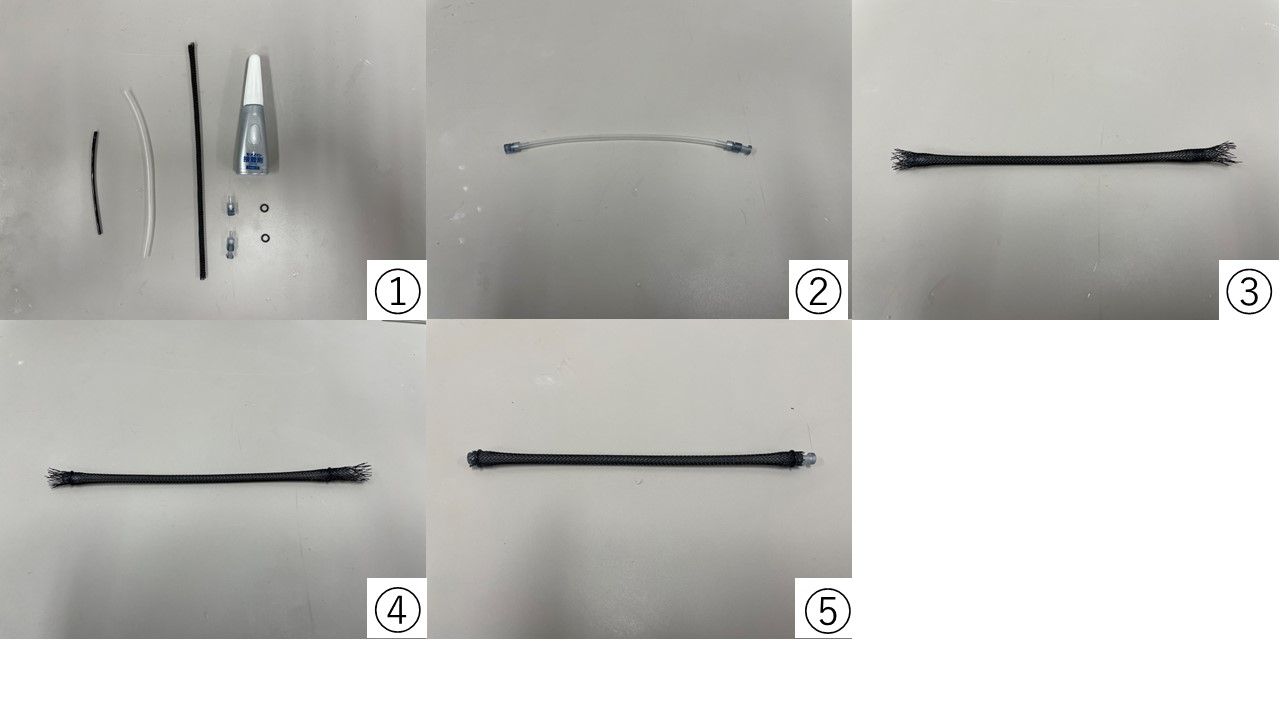
\includegraphics[scale=0.4]{image/sakusei.jpg}
  \caption{改良型細径MPAの作製方法}
  \label{fig:shingata_sakuseihouhou}
\end{figure}
%%%%%%%%%%%%%%%%%%%%%%%%%%%%%%%%%%%%%%%%%%%%%%%%%%%%%%%%%
\subsubsection{細径MPA締結方法の改善}
先行研究の細径MPA締結方法を図\ref{fig:MPA_tanbu_1}\subref{fig:MPA_tanbu_1_1}に示す.
%%%%%%%%%%%%%%%%%%%%%%%%%%%%%%%%%%%%%%%%%%%%%%%%%%%%%%%%%
\begin{figure}
  %
  \begin{minipage}{0.5\hsize}
    \centering  
    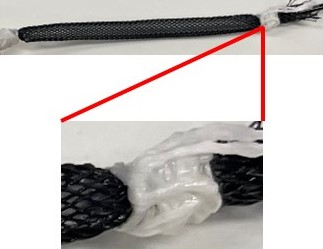
\includegraphics[scale=0.6]{image/MPA_tanbu_1_1.jpg}
    \subcaption{旧型細径MPA外観}
    \label{fig:MPA_tanbu_1_1}
  \end{minipage}
  %
  \begin{minipage}{0.5\hsize}
    \centering
    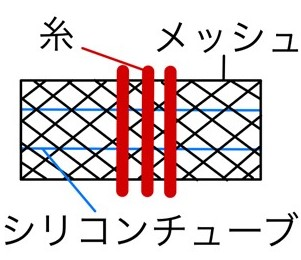
\includegraphics[scale=0.6]{image/MPA_tanbu_1_2.jpg}
    \subcaption{旧型細径MPA模式図}
    \label{fig:MPA_tanbu_1_2}
  \end{minipage}
  %
  \caption{先行研究で用いられた旧型細径MPA}
  \label{fig:MPA_tanbu_1}
\end{figure}
%
\begin{figure}
  %
  \begin{minipage}{0.5\hsize}
    \centering  
    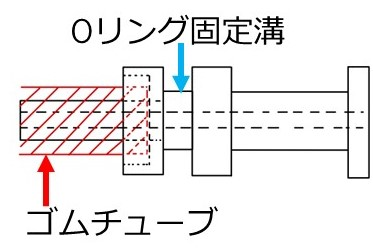
\includegraphics[scale=0.6]{image/MPA_tanbu_2_1.jpg}
    \subcaption{新型細径MPA外観}
    \label{fig:MPA_tanbu_2_1}
  \end{minipage}
  %
  \begin{minipage}{0.5\hsize}
    \centering
    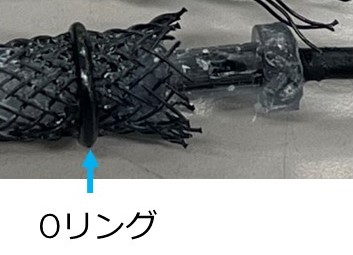
\includegraphics[scale=0.6]{image/MPA_tanbu_2_2.jpg}
    \subcaption{新型細径MPA模式図}
    \label{fig:MPA_tanbu_2_2}
  \end{minipage}
  %
  \caption{本研究で用いた新型細径MPA}
  \label{fig:MPA_tanbu_2}
\end{figure}
%%%%%%%%%%%%%%%%%%%%%%%%%%%%%%%%%%%%%%%%%%%%%%%%%%%%%%%%%
\subsubsection{細径MPA収縮率の向上}
市販に売られている編組チューブは,図\ref{fig:messhu_henka}\subref{fig:messhu_1}のように断面が平たく折癖がついている.
その状態の編組チューブを用いて細径MPAを作成すると,図\ref{fig:MPA_henka}\subref{fig:MPA_1}のようにシリコンゴムチューブと編組チューブの間に隙間が生じてしまう.
これにより,自身の径方向に膨張し軸方向に収縮する細径MPAにとっては収縮率を低下させる原因となる.
そこで本研究では,細径MPAの収縮性能を高めるために編組チューブを熱可塑変化させた.
大まかな作成方法をず\ref{fig:messhu_method}に示す.
図中\textcircled{\scriptsize 1}に示した物品が作製に必要なもので左から以下の通りである.
%
\begin{itemize}
  \item Oリング $\phi$ 4($\pm$ 0.15) メーカー:モノタロウ 品番:1A-SS 4.5
  \item ステンレス丸棒 $\phi$ 2mm メーカー:モノタロウ 品番:1378
  \item 編組チューブ 1×5(最小径×最大径) メーカー:モノタロウ 品番:-
  \item マスキングテープ テープ幅 15mm メーカー:モノタロウ 品番:15
  \item ホットプレート メーカー:山善 品番:YHA-W102
\end{itemize}
%
熱可塑変化の手順を以下に示す.
\vspace{3mm}
\begin{enumerate}
  \item まず初めに,編み込みチューブをステンレス棒よりも 3cm程短い範囲で任意の長さに切る
  \item 編み込みチューブにステンレス棒を差し込む(図中\textcircled{\scriptsize 2})
  \item 編み込みチューブの内径がステンレス棒の外径になるようにマスキングテープで巻いて固定する(図中\textcircled{\scriptsize 3})
  \item ホットプレートを 180℃まで温めて,編み込みチューブ全体に熱が伝わるように転がしながら3分間温める(図中\textcircled{\scriptsize 4})
  \item 全体を冷水に漬けて,3分間ほど熱をとる(図中\textcircled{\scriptsize 5})
  \item 粗熱が取れたらマスキングテープを外して完成
\end{enumerate}
熱可塑変化によって編組チューブは図\ref{fig:messhu_henka}のように折癖が取れ
%%%%%%%%%%%%%%%%%%%%%%%%%%%%%%%%%%%%%%%%%%%%%%%%%%%%%%%%%
\begin{figure}[ht]
  %
  \begin{minipage}{0.5\hsize}
    \centering  
    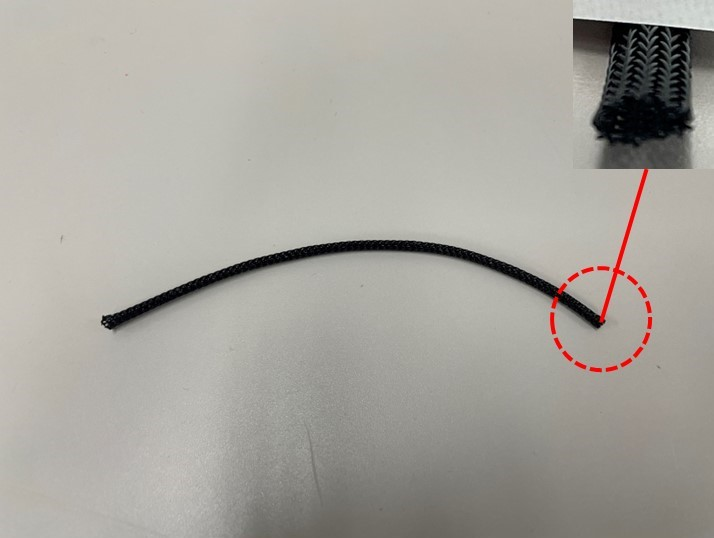
\includegraphics[scale=0.25]{image/messhu_hikaku_1.jpg}
    \subcaption{変化前}
    \label{fig:messhu_1}
  \end{minipage}
  %
  \begin{minipage}{0.5\hsize}
    \centering
    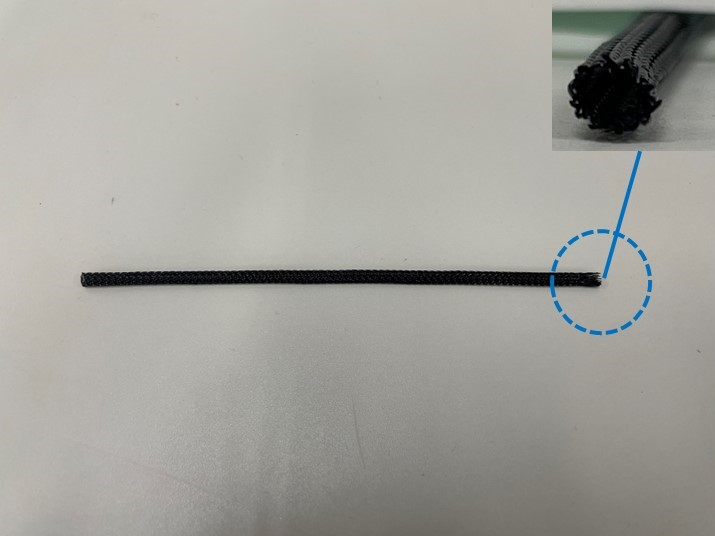
\includegraphics[scale=0.25]{image/messhu_hikaku_2.jpg}
    \subcaption{変化後}
    \label{fig:messhu_2}
  \end{minipage}
  %
  \caption{メッシュの熱可塑変化の様子}
  \label{fig:messhu_henka}
\end{figure}
%
\begin{figure}[ht]
  %
  \begin{minipage}{0.5\hsize}
    \centering  
    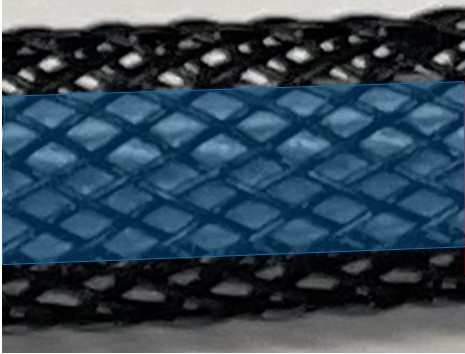
\includegraphics[scale=0.4]{image/hikaku_MPA_1.jpg}
    \subcaption{変化前}
    \label{fig:MPA_1}
  \end{minipage}
  %
  \begin{minipage}{0.5\hsize}
    \centering
    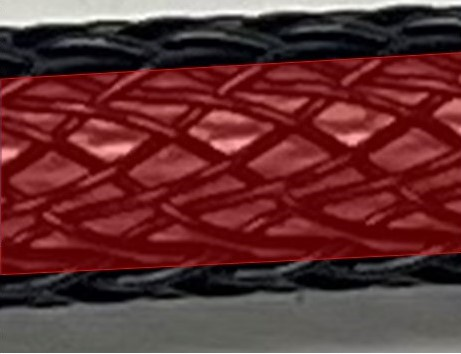
\includegraphics[scale=0.4]{image/hikaku_MPA_2.jpg}
    \subcaption{変化後}
    \label{fig:MPA_2}
  \end{minipage}
  %
  \caption{細径MPAの熱可塑変化の様子}
  \label{fig:MPA_henka}
\end{figure}
%
\begin{figure}[ht]
  \centering
  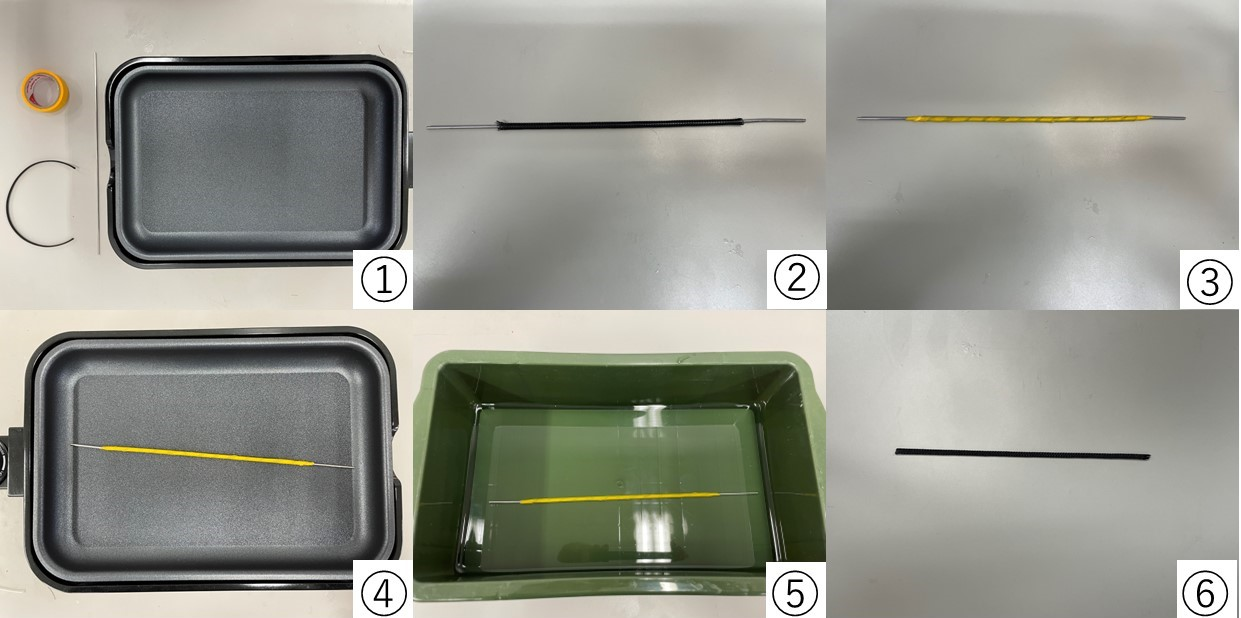
\includegraphics[scale=0.4]{image/messhu_tejyun.jpg}
  \caption{熱可塑変化の手順}
  \label{fig:messhu_method}
\end{figure}
%%%%%%%%%%%%%%%%%%%%%%%%%%%%%%%%%%%%%%%%%%%%%%%%%%%%%%%%%
\subsubsection{羽状角の自由度の再現}

%%%%%%%%%%%%%%%%%%%%%%%%%%%%%%%%%%%%%%%%%%%%%%%%%%%%%%%%%
\subsection{作製した機体}
\subsubsection{機体の構成および寸法}
%%%%%%%%%%%%%%%%%%%%%%%%%%%%%%%%%%%%%%%%%%%%%%%%%%%%%%%%%

